\section{Wellenleiter}
\subsection{Koaxialleiter}
\subsubsection{Wellenwiderstand}
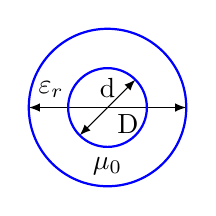
\begin{tikzpicture}
    \draw[latex-latex](-1,0)node[above right]{$\varepsilon_r$}--(1,0);
    \node[below right, yshift=1pt]{D};
    \draw[latex-latex, rotate=45](-0.5,0)--(.5,0);
    \node at (0,0)[above]{d};
    \draw[-, thick, blue](0,0) circle (1);
    \node at(0,-.75)[]{$\mu_0$};
    \draw[-, thick, blue](0,0) circle (0.5) ;
\end{tikzpicture}


D = Außendurchmesser

d = Innendurchmesser

\begin{align*}
    Z_L = \frac{60\Omega}{\sqrt{\varepsilon_r}}\cdot \ln{\frac{D}{d}}
\end{align*}

\subsubsection{Dämpfung}
\underline{\textbf{Ohm'sche Verluste}} $R\ll\omega L$
\begin{align*}
    \alpha_0 = \frac{\sqrt{\frac{f\cdot\mu}{\pi\cdot\sigma}}}{120\Omega}\cdot\frac{\sqrt{\varepsilon_r}}{D}\cdot\frac{1+\frac{D}{d}}{\ln \frac{D}{d}}
\end{align*}

\underline{\textbf{Dielektrische Verluste}} $G\ll\omega C$,$\tan\delta= (^G/_{\omega C})$
\begin{align*}
    \alpha_d = \pi\sqrt{\varepsilon_r}\cdot\tan\delta\cdot\frac{f}{c_0}
\end{align*}
